%\documentclass[11pt]{article}
\documentclass[11pt,a4paper]{tesis}
\usepackage[margin=1in]{geometry}          
\usepackage{graphicx}
\usepackage{subcaption}
\usepackage{placeins}
\usepackage{float}
\usepackage{amsthm, amsmath, amssymb}
\usepackage{setspace}\doublespacing
\usepackage[loose,nice]{units} %replace "nice" by "ugly" for units in upright fractions
\usepackage[
backend=biber,
maxbibnames=99,
sorting=none
]{biblatex}
\addbibresource{references_informe.bib}

\usepackage{hyperref}
\usepackage{csvsimple}
\usepackage{lscape}
\usepackage{hhline}
\usepackage[table,x11names]{xcolor}

\begin{document}
\linespread{1.6}
\tableofcontents
\chapter{Introduction}
	\section{Problem Description and Motivation}
		% % (REHACER UNA VEZ TERMINADAS LAS DEM\'AS SECCIONES DEL INFORME)

\section{Problem Description and Motivation} \label{section:motivation}

Technological improvements of last decades allowed the development and expansion of Computer
Assisted Language Learning (CALL) systems. These tools are aimed to help students along the
process of second language acquisition. One of the points where the
students should focus is in pronunciation learning, that usually requires a one-to-one teacher
interaction. Automatic pronunciation assessment is very useful in this
context because it provides an alternative way of learning with a performance close to human judgement,
cheaper and typically available at any time and any place.

% Pronunciation is a general term that covers a number of different aspects and can be measured
% with different features. A lot of work has been done in the area, and a good summary of
% existing research to date followed by remaining challenges can be found in
% \cite{where_we_are_go}.

% Sometimes is difficult to determine whether or not a
% pronunciation error is being made because there is no clear definition of right or wrong
% pronunciation. Rather there exists an antire scale ranging from unintelligible speech to
% native-sounding speech. Taking that into account, pronunciation errors can be divided into
% phonemic and prosodic error types. Examples of severe errors of the first type are
% phoneme substitution, deletion or insertion. Errors on the prosodic side can be
% categorized in terms of stress, rythm and intonation. This work is focused in phonemic
% error detection.

% Whenever performing pronunciation assessment, the smaller the unit the higher the
% uncertainty of the assessment. Currently, the most reliable estimates of pronunciation
% are obtained from paragraphs composed of several sentences, so that an evaluation of the
% speaker's overall pronunciation proficiency can be done. However, in order for the system
% to provide valuable feedback of the particular error that is being made an analysis at a
% much shorter level, like phone, is required. By following this approach, the exact error within
% a word can be identified.

When working in automatic pronunciation assessment an important decision to be taken is
whether or not considering L1, the native language of the learner, along the process. These
systems have improved speech recognition accuracy because they are designed
taking into account common known errors between L1 and L2. For example, native American English
students that are learning Spanish have difficulties pronouncing the diphtong [eu]
(e.g. ``eufemismo'') or
/r/ after [l] (e.g. ``alrededor''), [n] (e.g. ``sonrisa'') and [s] (e.g. ``disruptivo''),
which should be thrilled in all cases.
On the other hand, native Spanish students
that are learning English may have trouble pronouncing
different kind of vowels that are present in English
but not in the former. This approach, however, requires a labeled nonnative speech database
which is an expensive and time-consuming task, and
it is not feasible in some cases.
A database like that
is available
for the current thesis.
It contains collected
speech from native american english speakers that are learning
spanish, and it is used to train and test the different models.


% so different experiments are carried out using L1-based models, which
% are trained on collected speech from native american english speakers that are learning
% spanish.

% Whenever performing pronunciation assessment, the smaller the unit the higher the
% uncertainty of the assessment. Currently, the most reliable estimates of pronunciation
% are obtained from paragraphs composed of several sentences, so that an evaluation of the
% speaker's overall pronunciation proficiency can be done. However, in order for the system
% to provide valuable feedback of the particular error that is being made an analysis at a
% much shorter level, like phone, is required. By following this approach, the exact error within
% a word can be identified.

In the area of pronunciation scoring, the smaller the unit to be scored, the higher the
uncertainty in the associated score \cite{pronunciation_scoring_phone_segments_instruction}.
Currently, the most reliable estimates are obtained from paragraphs composed of several
sentences that can be used to characterize the speaker's overall pronunciation
proficiency \cite{main}. However, specific problems can be pointed out
when scoring smaller units, which is of great value because it allows the students to focus
on specific aspects of their speech production.

% This thesis is part of a bigger project led by Dr. Luciana Ferrer, whose objective is
% the development of a CALL system for Argentine children that are learning english. The goal
% is to generate pronunciation scores for students utterances at phone level. This way,
% all children may enjoy the benefits of using the system, including those who aren't capable
% of pronouncing entire paragraphs or long sentences due to lack of skills. In addition it will
% help to detect specific errors in the students pronunciation, so they can focus in that
% particular points when practicing the language.

% Even though the database for the current work uses American English as L1 and Spanish as L2,
% the same implementation can be used to train the main system of the global project once
% collected the children utterances.
% \underline{In the current thesis, a system based on L1 language is used to assess
% pronunciation of english speakers learning spanish}

The current work is part of a bigger project lead by Dra. Ferrer, with the objective
of developing a CALL system for Argentine children that are learning English.
The project has 3 main stages: The collection and annotation of a speech database
of Argentine children, the development of an \textit{Automatic Speech Recognition} (ASR) system and the development of a pronunciation scoring system that works at phone or word
level. The fact that the system works with short speech segments is specially important in
the context of a CALL system for children, because of the difficulty of children in
pronouncing longer segments.

In the current thesis, we based on L1 strategies to
explore alternatives to existing techniques in the
pronunciation assessment field at phone level. The explored
methods could be helpful
during the development of the CALL system for Argentine children that are learning English.

	\section{Previous work}
		In this section we will be reviewing representative works in pronunciation assessment
at phone level, which is the topic of interest in this thesis.

One of the simplest ways of scoring a phone pronunciation found in the literature 
is to use segment duration scores (\cite{pronunciation_scoring_instruction, pronunciation_scoring_phone_segments_instruction}), which are obtained through the following
procedure. First, a discrete duration distribution is generated for each phone
using the native training data. 
Then, phone durations in frames for nonnative utterances are obtained 
and its value is normalized to compensate for rate of speech. 
Finally, phone-segment-duration scores are computed as 
the log-probability of the normalized duration, using the discrete duration 
distributions previously mentioned. Phone durations are obtained from Viterbi alignments.
In the same works, other two methods that use \textit{Hidden Markov Models} (HMMs) to obtain 
spectral matches and compute pronunciation scores are tested. 
Phonetic time alignments for
non-native utterances are generated from an HMM-based speech recognition system trained
with native instances. In order to do that, the text pronounced by the student 
must be known. This is achieved by eliciting speech in a
constrained way, such as reading a predefined text.
From these phonetic segmentations two 
probabilistic mesasures based on HMMs are computed as scores: log-likelihood and 
log-posterior probabilities. The underlying asumption is that the logarithm of the likelihood
of the speech data, computed by the Viterbi algorithm using the HMMs trained with speech from native
speakers is a good mesasure of the similarity between the students's
speech and native-sounding speech.

For each phone segment the log-likelihood score \^{l} is computed as:
\begin{equation}
\hat{l} = \frac{1}{d} \sum_{t=t_{0}}^{t_{0}+d-1} log \ p(y_{t}|q_{i})
\end{equation}
where $p(y_{t}|q_{i})$ is the likelihood at the time $t$ with observation vector $y_{t}$
given the phone class $q_{i}$, $d$ is the duration in frames of the phone segment 
and $t_{0}$ is the starting frame index of the phone segment. Duration normalization is done to 
eliminate the dependency of the pronunciation score on the duration of the phone.

Alternatively, log-posterior scores can be computed for each time $t$:

\begin{equation}
P(q_{i}|y_{t}) = \frac{p(y_{t}|q_{i})P(q_{i})}{\sum\limits_{j=1}^{M} p(y_{t}|q_{j})P(q_{j})}
\end{equation}
Likelihood in the numerator is computed through a forced recognition phase by using a known 
ortographic transcription of the speech signal. On the other hand, 
the sum over $j$ runs over a set of context-independent models for all phone classes. $P(q_{i})$
represents the prior probability of the phone class $q_{i}$. 

Finally, the posterior score $\hat{\rho}$ for the phone segment is defined as:
\begin{equation}
\hat{\rho} = \frac{1}{d}\sum_{t=t_{0}}^{t_{0}+d-1} log \ P(q_{i}|y_{t})
\end{equation}

To test each method, a database of nonnative read speech is transcribed and scored for 
pronunciation quality by expert human raters. Log-posterior probabilities achieves the
highest correlation with human ratings, outperforming log-likelihood and normalized duration
scores.

A very similar approach to log-posterior probabilities named \textit{Goodness of Pronunciation}
(GOP) was developed at the same time as log-posteriors and
is used in some works \cite{gop_1, gop_2, gop_3}. The quality of 
pronunciation for any phone $p$ is defined to be the duration-normalized log of the posterior
probability that the speaker uttered phone $p$ given the corresponding vector of observations
$y=\{y_{t_{0}}, \dotsc y_{t_{0}+d-1} \}$

\begin{equation}
GOP(p) = \left| log \ \left(\frac{p(y|q)P(p))}{\sum_{q \in Q}p(y|q)P(q))}\right) \right| \Biggm/ d 
\end{equation}

The likelihoods $p(y|q)$ are obtained from the recognizer as a sum of the likelihoods over all
observations in the phone.
The difference between GOP scores and log-posterior score technique previously mentioned 
is that in GOP, the likelihood for both numerator and every phone in the denominator is
computed at segment level as a sum of log-likelihoods per frame over the 
duration of the phone $p$, while in Equation (1.2) log-posterior probabilities are computed
at the frame level and averaged over the segment's length.

So far, aforementioned methods are based on confidence measures 
obtained from Automatic Speech Recognition (ASR) systems. 
Scores measure how closely the utterance of the speaker matches the recognizer's
acoustic model. Mismatches result in low confidence scores, which provide a profile of the 
speakers' production erorrs. Nevertheless, the accuracy of the assessment based on these
confidence scores can be quite low \cite{landmark_svm}. 
In addition, ASR systems based on HMMs are both time-consuming to train and extremely vulnerable to
acoustic interference and variation in speaking style, and the conventional methods for
enhancing ASR performance often require enormous amounts of data collection and annotation,
as well as extensive training on representative material.
For those reasons, other types of classifiers are explored in many works, specially after
the 1990s. 

\textit{Support Vector Machines} (SVMs) are a preferred choice 
due to their excellent generalization capability and suitability for 2-class classification
problems. Moreover, in contrast to the confidence models described above, which do not take into
account misspronounced data, SVMs are trained directly to discriminate the two classes of interest.
Of course, this poses a new requirement: both correctly and incorrectly-pronounced data should be
available for training.

In \cite{detection_mispronunciation_dutch_vowel}, SVMs are trained with different types of
features to discriminate between good and mispronounced vowels in Dutch: log-posterior-based 
scores obtained from HMMs, MFCCs and a set of 
phonetic features (first three formants, pitch and intensity). Despite the existence of nonnative-speech  
databases for Dutch language, they were considered too small for the purpose of the research. 
For that reason, phonemic 
substitutions that induce vocalic errors are simulated by artificially introducing them in the native corpus.
The results show that the best 
results are obtained by using MFCCs as features of the SVM models, followed by confidence-measure-based 
scores and finally phonetic
features, though substantial improvements can be obtained by combining them.

In a different work \cite{svm_space_models}, SVM is used as the classifier and the
log-likelihood ratios between all the acoustic models and the model corresponding to the given
phone are employed as features for the classifier. In other words, given the observation
$y$, the feature vector for the classification problem is computed as:

[$LLR(y|q,q_{1}), \ LLR(y|q,q_{2}) \dotsc LLR(y|q, q_{M})$],

where $q$ is the canonical label of the observation being pronounced and {$q_{1}, q_{2} \dotsc q_{M}$}
represent the set of acoustic models of all the phones. The reason for choosing these features is
that $q$ can be mispronounced as any other phone and the likelihood ratio is a powerful
method to detect this kind of mispronunciation. Classifiers trained with this kind of features, however, 
can only effectively deal with a phone mispronounced as another phone. This kind of acoustic models is 
less effective for partially changed mispronunciations, that are the most frequent mispronunciations
in practice. In order to detect all kinds of mispronunciation, a technique called  
\textit{Pronunciation Space Models} (PSMs) is introduced. The idea is to represent pronunciation variations
of different proficiency levels. The traditional phone-based model $q$ is expanded to 
\{$q_{1}, q_{2} \dotsc q_{K}$\} representing $K$ types of pronunciation variations, ranging from perfect or
totally wrong pronunciations, where $K$ is a tunable parameter. PSMs are built from an unsupervised method
using the posterior probabilities obtained from the acoustic models for each phone $q$.
Experiments are carried out on the 
Mandarin mispronunciation detection task for native Chinese speakers with various dialect accents, 
and data labeled as 'correct' or not by experienced human annotators is used to train and test the models.
Results show that SVM based on log-likelihood ratio features outperforms GOP scores (used as baseline), and some
imporvements are obtained when adding PSMs.

Relying on labeled nonnative speech data usually leads to more flexible models 
with better performance than those trained with native speech
when working on pronunciation assessment for specific combinations of L1 and L2. On the one hand,
the set of common pronunciation errors tend to be particular for a given \textless L1, L2 
\textgreater \ pair so 
models that specifically focus on those errors can be trained. On the other hand, it provides more 
flexibility by assessing nonnative utterances that are close enough to native-sounding as correct, 
in a similar way that an annotator would do. 
However, labeled nonnative speech databases are rarely available. Both collection and annotation 
of nonnative speech is an expensive and time-consuming task, and in some cases it is not feasible.
So models trained with annotated nonnative speech usually have better performance
than those trained with native data, though the cost of non-native database 
collection and annotation is very high.

Finally, a last example of SVM-based resarch is found in \cite{landmark_svm, landmark_svm_2}. 
A landmark-based SVM is introduced and compared with a confidence 
scoring method over 10 phonemes where 
L2 English learners, whose native language is Korean, make frequent errors. 
Landmark theory relies on the fact that humans can perceive distinctive
features using only spectral features extracted from the time frame including and adjacent to
a landmark (sudden signal change). A particular SVM for each phoneme is trained. Vowel SVMs are 
trained using one or more frames from the vowel center. Frames from both onset and offset
(prevocalic and postvocalic position) are selected and used in the training of consonant
SVMs. The confidence score method shows a similar performance to SVM, though by combining 
the two scores, statistically significant improvements are achieved for almost all phonemes.

A different strategy for discrimination of Dutch velar fricative /x/ versus the velar plosive
/k/ is studied in \cite{lda_weigelt}. Latent Discriminant Analysis (LDA) over two different sets
of features are explored and compared with previous approaches: aforementioned GOP scores and
Weigelt algorithm. The latter is based on three measures that can be easily obtained:
log root-mean-square (rms) energy, the derivative of log rms energy (\textit{Rate of Rise} or
ROR) and zero-crossing rate. Weigelt algorithm discriminate plosives from fricatives by using
ROR values, based on the fact that the release of the burst of the plosives causes an abrupt
rise in amplitude therefore yielding higher values compared with fricatives.
On the other hand, LDA weights are assigned to each feature to 
find the linear combination of features
which best separates the classes. Selecting the most relevant features turns out to give an
advantage compared to other classifiers. The two LDA methods yielded the best performing
scores followed by GOP and Weigelt.

A second group of papers are based on L1 strategies. A sufficiently large annotated nonnative
database is required in order to follow approaches of this kind.
In \cite{detection_phone_level_mispronunciation_learning}, a phonetically labeled nonnative
database is used to train two different \textit{Gaussian mixture models} (GMMs) for each phone
class: one model is trained with the "correct" native-like pronunciations of a phone, while the
other model is trained with the "mispronounced" or nonnative pronunciations of the same phone.
In the evaluation phase, for each phone segment $q_{i}$, a length-normalized log-likelihood ratio
$LLR(q_{i})$ score is computed for the phone segment by using the "mispronounced" and "correct"
pronunciation models $\lambda_{M}$ and $\lambda_{C}$ respectively:
\begin{equation}
LLR(q_{i}) = \frac{1}{d}\sum_{t=t_{0}}^{t_{0}+d-1} [log \ p(y_{t}|q_{i}, \lambda_{M}) - log \ p(y_{t}|q_{i}, \lambda_{C})]
\end{equation}
The normalization by $d$ allows definition of unique thresholds for the LLR for each phone class, 
independent of the length of the segments.

Finally, a recent work \cite{main} explores another method that also uses 
log-likelihood ratio based on  GMMs (eq 1.4), except that the models for each 
class ("correct" and  "mispronounced") are obtained by adaptation. In the same work, 
a discriminative system based
on \textit{Support Vector Machines} (SVM) is developed producing good results. Features 
for this classifier are obtained by adapting class-independent GMMs to each particular 
instance of the target phone and extracting both means and weights of the resulting 
Gaussian Mixture.
These methods proved to be superior to the mispronunciation detection system based of 
LLR of independently trained GMMs (eq 1.4), which had been previously shown to 
outperform the standard method tha uses phone log-posterior as scores, yielding
results comparable to state-of-the-art techniques.
Both systems previously described are used as baselines in the work here 
presented so a detailed explanation will be provided in next sections.

\chapter{Method}
	% \begin{itemize}
	\item Gaussian Mixture Model
	\item Log Likelihood Ratio method to asses pronunciation
	\item GMM adaptation method
	\item Generating supervectors from adapted GMMs
\end{itemize}
	In this section we will review the way the pronunciation scoring system works
and explain the concepts and techniques on which it is based. The diagram below
shows the overall architecture of the system:

~

\begin{figure}[H]
	\centering
	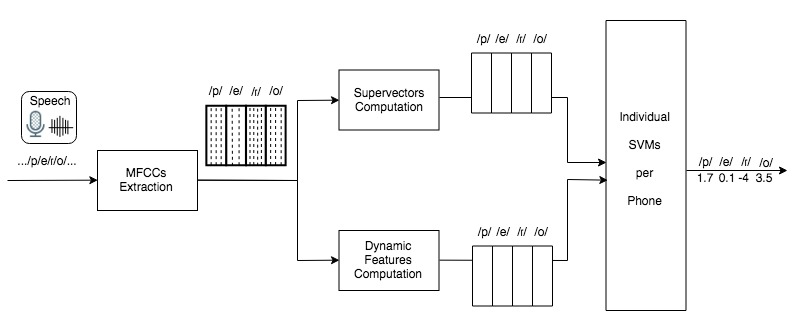
\includegraphics[width=0.9\textwidth]{files/figures/method/general-structure-v2.jpg}
	\caption{General System Architecture}
	\label{fig:methodGeneralArchitecture}
\end{figure}

Given a test instance, the objective is to compute a score for each phone that
is uttered in that instance. In order to do so, the flow goes as follows:

\begin{enumerate}

 \item The first step is to calculate the audio features from the recordings.
 This is done in order to summarize the signal information
 in a measurable way through numeric values. The chosen features
 are the \textit{Mel Frecuency Cepstral Coefficients} (MFCCs) because they are one of the
 most standard and widely-spread features in the speech processing field.

 \item The MFCCs are then split in segments according to the phones to which they
 belong. Each segment is at the same time divided in frames, that represent short
 intervals where the audio signal is not supposed to be changing so much.

 \item MFCCs of each phone instance present in the utterance
 are then used to compute the more complex phone-level features
 on which the SVMs operates. Supervectors are the base and proven to work features,
 while the Dynamic Features are the experimental features to be studied.

 \item {
  SVM classifiers are trained individually for each phone. Two alternative ways of combining the
  features are studied:
    \begin{itemize}
      \item Training a single SVM from a combination of both Supervectors and Dynamic Features.
      \item Training two separate SVMs: one using the Supervector features while the other using the
      Dynamic Features, and then combining the results.
    \end{itemize}
 }

 \item Finally an individual score is obtained for each of the instances
 of the different phones present in the
 utterance. Phone instances with positive score are labelled as
 correct while phone instances with negative score are labelled as incorrect.
 The bigger the magnitude of the score, the more sure the system is about the
 decision.

\end{enumerate}


	\section{Features}
		\subsection{Feature Extraction}
		The first step in order to build the system is to extract features from the speech data.
The feature extraction process aims at approximating the linguistic content that is conveyed
by the speech signal, by identifying its relevant aspects and discarding other unuseful
properties like background noise, emotions, etc.

\subsection{MFCCs Extraction}
In this work we base our features in the standard and widely used Mel Frecuency
Cepstral Coefficients (MFCCs). They were introduced by Davis and Mermelstein in 1980 and
have been state-of-the-art ever since \cite{mfcc_foundational}.
MFCC coefficients represent the spectral envelope of the speech signal on the Mel-frequency scale,
which relates the perceived frequency of a pure tune to its actual measured frequency inspired
by the human hearing.

The process to compute the MFCCs coefficients can be summarized into applying the following steps:

\begin{enumerate}

  \item Preemphasis: Preemphasis aims at increasing the amplitude of high frequency bands while
  decreasing the amplitudes of lower bands by means of a high-pass filter. This stage is performed
  in order to balance the frequency spectrum since high frequencies usually have smaller
  magnitudes compared to lower ones.
  % http://haythamfayek.com/2016/04/21/speech-processing-for-machine-learning.html
  % https://www.quora.com/Why-is-pre-emphasis-i-e-passing-the-speech-signal-through-a-first-order-high-pass-filter-required-in-speech-processing-and-how-does-it-work

  \item Windowing: The MFCCs are computed in time intervals where the audio signal isn't
  supposed to be changing
  so much. Because of that reason the signal is divided in frames using a
  25 ms duration window and 10 ms shift (standard values). A 25 ms duration window provides
  enough samples to get a reliable spectral estimate: 200 samples per frame at 8 $kHz$,
  and at the same time is short enough to minimize the signal changes.
  On the other hand, a 10 ms shift leads to a
  15 ms overlap between consecutive frames, ensuring that the information between adjacent
  frames is also captured in the middle of another frame.
  % http://practicalcryptography.com/miscellaneous/machine-learning/guide-mel-frequency-cepstral-coefficients-mfccs/

  \item Discrete Fourier Transform: This is the first and main step in regard to spectral
  analysis. Frequency domain approaches are proven to be
  among the best options in speech classification tasks.
  The \textit{spectral density}, which is the distribution of power
  into the frequency components composign the signal, is obtained for each frame by using
  the Discrete Fourier Transform technique.   % mfcc_extraction_v3

  \item Mel Filter-bank: At this stage, a perceptual scale of pitches inspired in human
  hearing called Mel scale is used. Because humans are much better at discerning small changes
  in pitch at low frequencies than they are at high frequencies,
  the Mel frequency scale is linear up to 1000Hz and logarithmic thereafter according to
  the following formula:

  \begin{equation}
    M(f)=1125*ln(1 + \frac{f}{700})
  \end{equation}

  The spectrum obtained in (3) is passed through a series of traingular filters
  uniformly spaced on the Mel scale to produce the so called filter-bank energies.
  The original values of these energies are replaced by their natural logarithm values,
  also motivated by human hearing: loudness is not perceived according to
  a linear but an exponential scale.

  \item Cepstral Coefficients: The Discrete Cosine Transform (DCT) is applied to the logarithm
  of the filterbank energies to obtain the Cepstral Coefficients. In general, only the lower
  12 Cepstral Coefficients are kept. The resulting features are called Mel Frequency
  Cepstral Coefficients. Additionally, a $13\textsuperscript{th}$ MFCC computed
  as the sum of the energy in the frame is included,
  because it usually improves the performance in phone detection
  related tasks.

  \item Deltas and Double Deltas: Finally, the speech also carries information
  in the dynamics, i.e, trajectories of the MFCC coefficients over time. Calculating
  the MFCC trajectories and appending them to the original MFCC vector usually increase the
  performance of the systems. Both Delta and Delta-Delta features are included, adding to
  a total of 39 features per frame.

  \end{enumerate}

			% \subsubsection{Windows and Shifts}
			% \subsubsection{Mel-Frecuency Cepstral Coefficients}
			% 	\begin{itemize}
	\item Description. What are Mel Frequency Cepstral Coefficients?
	\item Normalization technique
	\item Motivation for varying window and shift
\end{itemize}
		% \subsection{Cepstral Mean Substraction}
	\section{Gaussian Mixture Model}
		\subsection{Definition}
		\subsection{GMM Adaptation}
		\subsection{Log-Likelihood Ratio Method}
	\section{Support Vector Machines}
		The chosen model for the discriminative analysis is the \textit{Support Vector Machine} classifier,
an approach for classification that was developed in the computer science community in the 1990s
and that has grown in popularity since then. The SVM is a member of the family of
\textit{maximal margin classifiers}, which base its strategy in finding the hyperplane that
best separate the positive and negative instances \cite{svm_jwht}.

\subsection{Maximal Margin Classifiers}
In a \textit{p-dimensional} space, a hyperplane is a flat affine subspace of
dimension $p-1$ defined by the equation:

\begin{equation}
  \label{eq:hyperplane}
  \beta_{0} + \beta_{1}X_{1} + \beta_{2}X_{2} + \dotsc + \beta_{p}X_{p} = 0
\end{equation}

The equation defines a \textit{p-dimensional} hyperplane in the sense that if a point
$X=(X_{1}, X_{2}, \dotsc, X_{p})^{T}$ in \textit{p-dimensional} space
satisfies \ref{eq:hyperplane} then $X$ lies on the hyperplane.

If $X$ doesn't lie in the hyperplane then either:

\begin{equation}
  \label{eq:hyperplaneGreater}
  \beta_{0} + \beta_{1}X_{1} + \beta_{2}X_{2} + \dotsc + \beta_{p}X_{p} > 0
\end{equation}

\begin{center}or\end{center}

\begin{equation}
  \label{eq:hyperplaneLesser}
  \beta_{0} + \beta_{1}X_{1} + \beta_{2}X_{2} + \dotsc + \beta_{p}X_{p} < 0
\end{equation}

So the hyperplane somehow divides the \textit{p-dimensional} space into two halves. One can
easily determine on which side of the hyperplane a point lies by simply calculating the sign
of the left hand side of \ref{eq:hyperplane}.

Having a set of $n$ instances of dimension $p$, with labels
$y_{1}, y_{2}, \dotsc y_{n} \in \{-1,1\}$ and $x^{i} = (x^{i}_{1}, x^{i}_{2}, \dotsc x^{i}_{p}) \ \forall \ 1 \leq i \leq {n}$ and supposing that it is possible to construct a hyperplane that
separates the training observations perfectly according to their class labels, then a
separating hyperplane has the property that:

\begin{equation}
\beta_{0} + \beta_{1}X_{1} + \beta_{2}X_{2} + \dotsc + \beta_{p}X_{p} > 0 \ if \ y_{i} = 1
\end{equation}

\begin{center}and\end{center}

\begin{equation}
\beta_{0} + \beta_{1}X_{1} + \beta_{2}X_{2} + \dotsc + \beta_{p}X_{p} < 0 \ if \ y_{i} = -1
\end{equation}

A test observation $x^{*}$ is classified based on the sign of
$f(x^{*})=\beta_{0}+\beta_{1}x^{*}_{1} + \beta_{2}x^{*}_{2} + \dotsc + \beta_{p}x^{*}_{p}$.
If $f(x^{*})$ is positive, then it is assigned to class 1 whereas if $f(x^{*})$ is negative
then it is assigned to class -1. In addition, the magnitude of $f(x^{*})$ also contains valuable
information.
If $f(x^{*})$ is far from zero then it means that $x^{*}$ lies far from the hyperplane
whereas if $f(x^{*})$ is close to zero then $x^{*}$ is located near the hyperplane and
there is less certainty about the class of $x^{*}$.

In general, if the data can be perfectly separated using a hyperplane, then there will be an
infinite number of such hyperplanes. This is because a given separating hyperplane can usually
be shift a tiny bit up or down, or rotating without coming into contact with any of the
observations.

\begin{figure}[H]
  \centering
  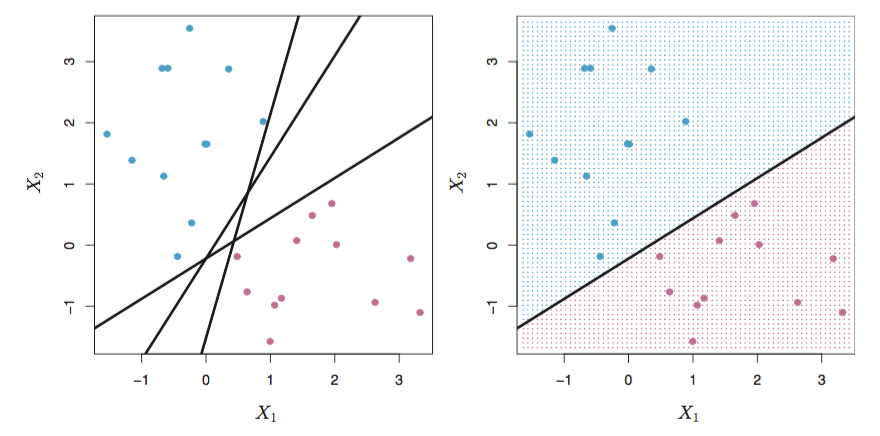
\includegraphics[width=0.8\textwidth]{files/figures/method/max-margin}
  \caption{Taken from \textit{JWHT} \cite{svm_jwht} book.
  Left: Three separating hyperplanes out of many
  possibilities. Right: Optimal Separating Hyperplane for the same dataset. A test observation
  that falls in the blue portion of the grid will be assigned to the blue class, and a test
  observation that falls in the purple portion of the grid will be assigned
  to the purple class.}
  \label{fig:maxMargin}
\end{figure}

A natural choice is the \textit{Maximal Margin Classifiers} (also known as the
\textit{Optimal Separating Hyerplane}), which is the separating hyperplane that is farthest
from the training observations. The \textit{margin} of the hyperplane is computed as the
minimal perpendicular distance to the hyperplane among all the training observations.
The maximal margin hyperplane is the separating hyperplane for which the margin is the largest.
The core idea is that a classifier that has a large margin on the training data will also
have a large margin on the test data.

\subsection{Support Vectors}

The separating hyperplane is determined by the instances of both classes that lies on the margin
of the hyperplane. These observations are known as \textit{Support Vectors}.
Observations can be interpreted as vectors in a \textit{p-dimensional} space and they
"support" the maximal
margin hyperplane in the sense that if these points were moved slightly then the maximal
margin hyperplane would move as well. The maximal margin hyperplane depends directly on the
support vectors, but not on the other observations: a movement to any of the other observations
would not affect the separating hyperplane, provided that the observation's movement does not cause
it to cross the boundary set by the margin.

\begin{figure}[H]
  \centering
  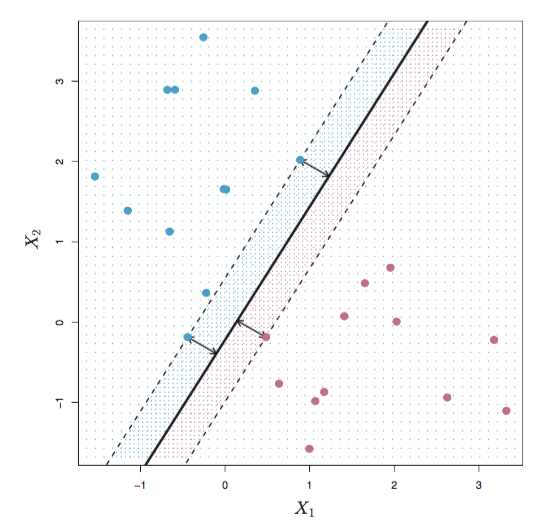
\includegraphics[width=0.4\textwidth]{files/figures/method/support-vectors}
  \caption{Taken from \textit{JWHT} \cite{svm_jwht} book. The maximal margin hyperplane
  is shown as a solid line. The margin is the distance between the solid line to either
  of the dashed lines. The two blue points and the purple point that line on the
  dashed lines are the support vectors.}
  \label{fig:maxMargin}
\end{figure}

\subsection{Problem Formulation}

It can be proven that given a set of $n$ observations of dimension $p$, the problem of
finding the \textit{Maximal Margin Hyperplane} can be posed as an optimization problem:
minimize $\| w \| = (\beta_{1}, \dotsc, \beta_{p})$.

\begin{equation}
\label{eq:svmOptimization}
w^{T}x^{*} = p\| w \|
\end{equation}

where $x^{*}$ is an observation and $p$ is the length of the projection of the observation
onto the normal vector of the hyperplane, i.e, the distance to the hyperplane.
Equation \ref{eq:svmOptimization} states that in order to maximize $p$ the norm of $w$
has to be minimized. On the other hand, the minimization problem is subject to the constraint:

\begin{equation}
  \label{eq:svmConstraint}
  y_{i} * (\beta_{0} + \beta_{1}x_{1} + \beta_{2}x_{2} + \dotsc + \beta_{p}x_{p}) > 0 \ \forall \ 1 \leq i \leq {n}
\end{equation}

Equation \ref{eq:svmConstraint} can be easily derived from \ref{eq:hyperplaneGreater} and
\ref{eq:hyperplaneLesser}.  This context matches the necessary conditions to apply
the \textit{Lagrange Multipliers} technique, to get this problem into a form
that can be solved analytically.

In practice, real data is scarcely ever completely linearly separable
and there is a trade off between
minimizing $\| w \|$ (i.e separating the instances by the largest possible margin)
and satisfying the constraint imposed over every
observation to lie on the right side of the hyperplane.
The desired hyperplane is one which separates correctly the vast majority of the observations and
at the same time it separates them by the largest margin. For this reason, when training an
\textit{SVM} classifier an additional parameter $C$ is passed as argument to the training
method in order to prioritize one problem over the other. A bigger $C$ favors the correctly
classification of the instances, while a smaller one favors the minimization of $\| w \|$
and thus finding the hyperplane with the largest margin for most of the instances.

(Agregar foto del efecto del parámetro C)

(Agregar la aclaración de que no vamos a comentar acerca de los kernels no lineales porque
no se usan)

		\subsection{Cost Function}
			\begin{itemize}
	\item Formula: $C*\displaystyle\sum_{i=1}^{m} [y^{(i)} * cost_{1}(\theta^{T} * x^{(i)}) + (1-y^{(i)}) * cost_{0}(\theta^{T} * x^{(i)}))] + \frac{1}{2} * \displaystyle\sum_{j=1}^{n} \theta^{2}_{j}$
	\item Formula description. Least square term vs regularization term
\end{itemize}
		\subsection{C Parameter}
			\begin{itemize}
	\item Explanation: How does it affect to the equation?
	\item Consequences of using a small $C$
	\item Consequences of using a large $C$
\end{itemize}
		\subsection{Balancing Class Weights}
			\begin{itemize}
	\item Behaviour and consecuences of classifier if no action is taken when dealing with unbalanced data
	\item Solution for unbalanced data problem
\end{itemize}
		\subsection{Feature Combination}
	\section{Legendre Polynomials}
		\subsection{Definition}
		\subsection{Least Squares}
		\subsection{Lasso Regression}
	\section{Discrete Cosine Transform}
	\section{Performance Measures}
		\subsection{ROC Curve}
		\subsection{Equal Error Rate}
			In order to measure the performance of the different systems, the \textit{Equal Error Rate} metric
is chosen. As its name suggests, the \textit{EER} prioritizes in an equal manner the
\textcolor{red}{
  \textit{False Positive Rate} and the \textit{False Negative Rate}.
}
This metric was used
in the previous works of the current line of investigation related to pronunciation assessment
at phone level \cite{detection_phone_level_mispronunciation_learning, main}, so the same approach
was taken in the present work.

The process for evaluating the performance of a classifier usually involves the following steps:
At first, the decision function of the classifier, which can be for example predicted probabilities
or in our case distances to the hyperplane, is computed for each instance of the test set.
Then, the obtained results are used to generate
a distribution of the instances count as function of the values
in the domain of the decision function. Finally,
in order to make class predictions a threshold is chosen and the instances with a result of the
decision function above that threshold are classified as positive, while
those with results below the threshold are classified as negative. Most classifiers
usually set a threshold by default, such as 0 in the case of Support Vector Machines that
determines a separation of
positives and negative instances according to the sign of their distance to the hyperplane.

The EER can be found by sweeping the threshold until reaching the condition that
False Positive Rate (FPR) equals False Negative Rate (FNR). FPR is computed as
\textcolor{red}{the proportion} of negative instances wrongly
categorized as positive: $\frac{FP}{TN+FP}$.
Analogously, FNR is computed as \textcolor{red}{the proportion} of positve
instances wrongly categorized as negative:
$\frac{FN}{TP+FN}$. A simple example of EER threshold is
shown in Fig. \ref{fig:eer}.

\begin{figure}[H]
  \centering
  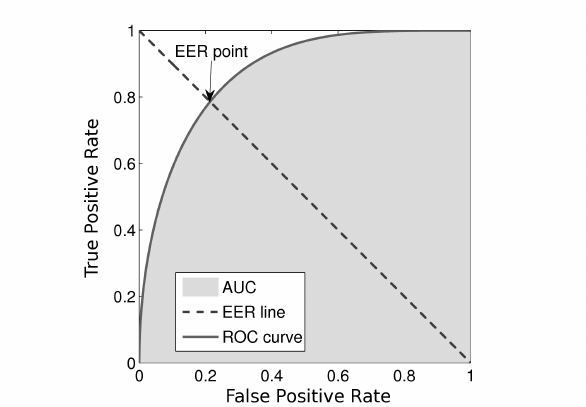
\includegraphics[width=0.8\textwidth]{files/figures/method/eer}
  \caption{An example of EER threshold with perfectly balanced classes. Both negative and positive distributions have the same size and shape.
  The threshold separates the instances in such way that FPR equals FNR.}
  \label{fig:eer}
\end{figure}

% Even though the diagram shows a case where the classes are perfectly balanced, in most of
% real world problems (including the current one) this does not happen. Distributions of both
% classes usually differs in both size and shape. However,
% as the technique is based on the \textit{rate} of misclassified positive and negative instances,
% the EER method can be applied without any trouble for unbalanced datasets and
% is computed exactly the same way: by sweeping the threshold until finding the point
% where FPR equals FNR.

	\section{Statistical Significance Techniques}
		\subsection{Bootstrapping}
		\subsection{McNemar}

\chapter{Experimental Design}
	\section{Architecture Overview}
		(Los siguientes diagramas fueron extraídos del toolkit description. 
La idea es armar unos nuevos propios con descripciones en inglés)

\begin{figure}[H]
	\centering
	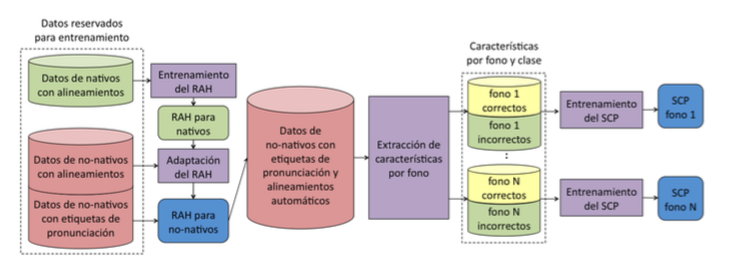
\includegraphics[width=0.7\textwidth]{files/figures/experimental_design/diagrama-1.png}
\end{figure}

\begin{figure}[H]
	\centering
	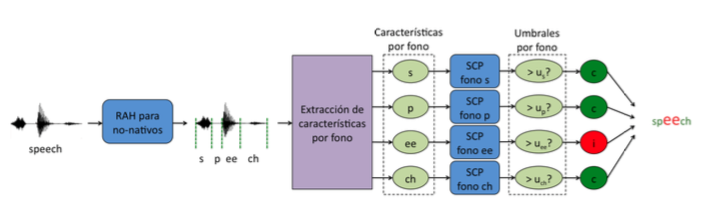
\includegraphics[width=0.7\textwidth]{files/figures/experimental_design/diagrama-2.png}
\end{figure}


	\section{Database Description}
	\section{Development and Test Sets Definition}
	\section{GMMs Experiments}
		\subsection{Independently-trained models}
		\subsection{Adapted models}
	\section{SVM Experiments}
		\subsection{Supervectors}
		\subsection{Legendre}
			\begin{itemize}
	\item Modeling time dependencies
	\item Difference with Supervectors obtained from GMM adaptation
\end{itemize}
		\subsection{DCT}
		\subsection{Features Combination}
		\subsection{Score Combination}

\chapter{Results}
	\section{GMM vs Supervectors}

[GMM vs supervectors] Adapt K-Means

\begin{figure}[H]
	\centering
	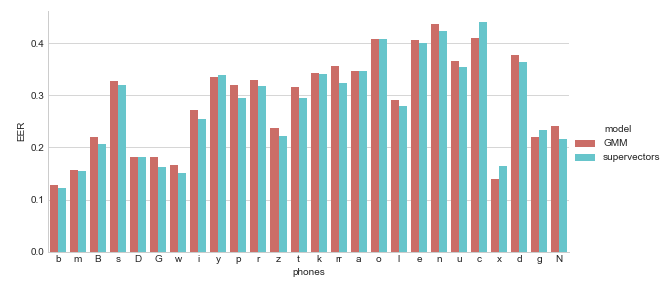
\includegraphics[width=0.6\textwidth]{files/figures/results/gmm-vs-supervectors/gmm-vs-supervectors-dev.png}
\end{figure}

\begin{figure}[H]
	\centering
	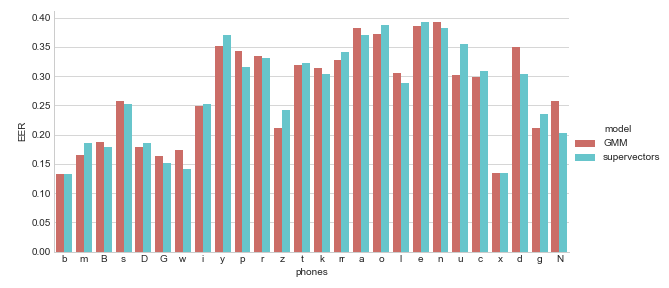
\includegraphics[width=0.6\textwidth]{files/figures/results/gmm-vs-supervectors/gmm-vs-supervectors-heldout.png}
\end{figure}


\section{Legendre Best System}

\begin{figure}[H]
	\centering
	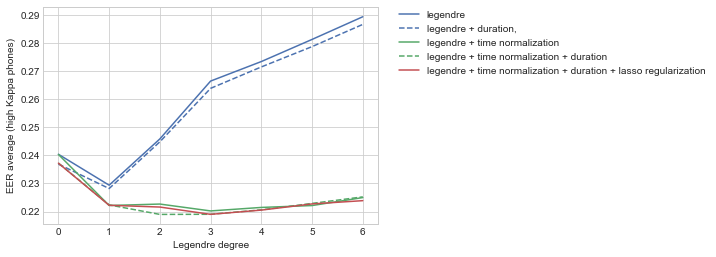
\includegraphics[width=0.8\textwidth]{files/figures/results/legendre-dct/legendre-tunning.png}
\end{figure}


\section{Legendre vs DCT}

\begin{figure}[H]
	\centering
	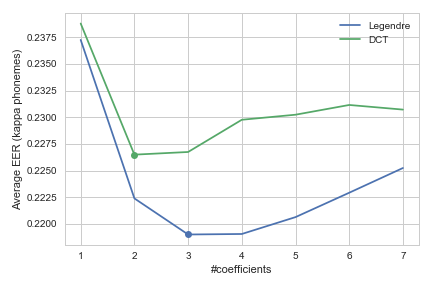
\includegraphics[width=0.5\textwidth]{files/figures/results/legendre-dct/legendre-dct-coefficients.png}
\end{figure}


\section{Fusion systems}

\subsection{Statistical Significant Filtering}

\subsection{Plots}

\begin{figure}[H]
	\centering
	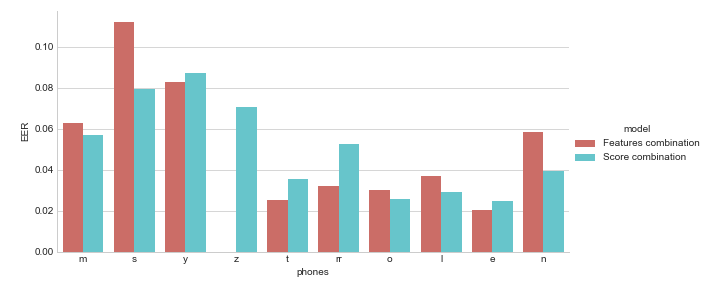
\includegraphics[width=0.6\textwidth]{files/figures/results/relatives/relatives-fusion-systems-dev-kappa.png}
\end{figure}

\begin{figure}[H]
	\centering
	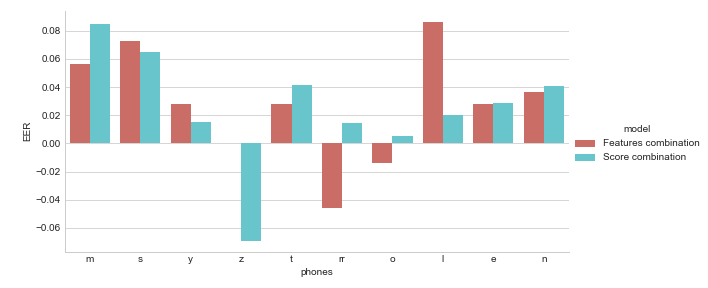
\includegraphics[width=0.6\textwidth]{files/figures/results/relatives/relative-fusion-systems-heldout-kappa.png}
\end{figure}


\chapter{Conclusions}
	\section{Improvements by Adding Dynamic Features}
	\section{Comparing Robustness of Fusion Systems}

\chapter{Appendix A}
	\section{Results Tables for All Phones}
		% --------------------------------------------------------------------------------%
% ---------------------------- Features combination ------------------------------% 
% --------------------------------------------------------------------------------% 
\subsection{Features combination}

\begin{table}[H]
\tiny{
\centering
\renewcommand{\arraystretch}{2}

\begin{tabular}{|c| |c|c|c|c|c|c| |c|c|c|c|c|c| |c|}
\hline
phones & baseline & training & delta & pvalue & \#pos & \#neg & baseline & test & delta & pvalue & \#pos & \#neg & kappa \\ \hline
b & 0.122 & 0.122 & \%0.0 & 1 & 528 & 395 & 0.133 & 0.133 & \%0.0 & 1 & 140 & 95 & 0.9 \\ \hline
\rowcolor{lightgray} m & 0.154 & 0.144 & \%6.5 & 0.047 & 3234 & 686 & 0.186 & 0.176 & \%5.4 & 0.268 & 801 & 188 & 0.76 \\ \hline
B & 0.206 & 0.2 & \%2.9 & 0.374 & 428 & 1169 & 0.179 & 0.189 & -\%5.6 & 0.523 & 126 & 302 & 0.7 \\ \hline
\rowcolor{lightgray} s & 0.319 & 0.283 & \%11.3 & 8.32E-19 & 7555 & 480 & 0.252 & 0.234 & \%7.1 & 0.454 & 1963 & 107 & 0.57 \\ \hline
D & 0.182 & 0.182 & \%0.0 & 1 & 920 & 2009 & 0.185 & 0.185 & \%0.0 & 1 & 268 & 486 & 0.55 \\ \hline
G & 0.162 & 0.162 & \%0.0 & 1 & 222 & 643 & 0.152 & 0.152 & \%0.0 & 1 & 61 & 145 & 0.51 \\ \hline
w & 0.151 & 0.151 & \%0.0 & 1 & 743 & 500 & 0.141 & 0.141 & \%0.0 & 1 & 179 & 128 & 0.43 \\ \hline
i & 0.254 & 0.252 & \%0.8 & 0.481 & 4929 & 1238 & 0.252 & 0.256 & -\%1.6 & 0.714 & 1224 & 301 & 0.41 \\ \hline
\rowcolor{lightgray} y & 0.338 & 0.31 & \%8.3 & 2.02E-05 & 2453 & 574 & 0.371 & 0.361 & \%2.7 & 0.844 & 596 & 156 & 0.39 \\ \hline
p & 0.295 & 0.295 & \%0.0 & 0.715 & 1657 & 1055 & 0.315 & 0.316 & -\%0.3 & 1 & 441 & 254 & 0.36 \\ \hline
r & 0.317 & 0.315 & \%0.6 & 0.561 & 3650 & 2617 & 0.331 & 0.315 & \%4.8 & 0.046 & 910 & 641 & 0.36 \\ \hline
z & 0.222 & 0.222 & \%0.0 & 1 & 189 & 997 & 0.242 & 0.242 & \%0.0 & 1 & 49 & 247 & 0.35 \\ \hline
t & 0.295 & 0.288 & \%2.4 & 0.183 & 2938 & 1542 & 0.323 & 0.314 & \%2.8 & 0.207 & 733 & 360 & 0.34 \\ \hline
k & 0.341 & 0.335 & \%1.8 & 0.339 & 1708 & 1472 & 0.304 & 0.305 & -\%0.3 & 0.913 & 434 & 388 & 0.32 \\ \hline
rr & 0.324 & 0.314 & \%3.1 & 0.299 & 491 & 1739 & 0.341 & 0.357 & -\%4.7 & 0.359 & 122 & 453 & 0.29 \\ \hline
a & 0.346 & 0.345 & \%0.3 & 0.712 & 10144 & 2069 & 0.371 & 0.354 & \%4.6 & 0.041 & 2509 & 548 & 0.26 \\ \hline
\rowcolor{lightgray} o & 0.408 & 0.396 & \%2.9 & 0.002 & 8040 & 2077 & 0.387 & 0.392 & -\%1.3 & 0.598 & 2030 & 548 & 0.23 \\ \hline
\rowcolor{lightgray} l & 0.279 & 0.269 & \%3.6 & 0.019 & 3505 & 1373 & 0.289 & 0.264 & \%8.7 & 0.009 & 851 & 356 & 0.22 \\ \hline
\rowcolor{lightgray} e & 0.4 & 0.392 & \%2.0 & 0.022 & 10597 & 3484 & 0.392 & 0.381 & \%2.8 & 0.095 & 2658 & 899 & 0.18 \\ \hline
\rowcolor{lightgray} n & 0.424 & 0.399 & \%5.9 & 1.27E-04 & 7152 & 476 & 0.382 & 0.368 & \%3.7 & 0.772 & 1792 & 125 & 0.15 \\ \hline
u & 0.354 & 0.344 & \%2.8 & 0.296 & 1948 & 482 & 0.355 & 0.336 & \%5.4 & 0.308 & 471 & 110 & 0.14 \\ \hline
x & 0.164 & 0.164 & \%0.0 & 1 & 590 & 153 & 0.135 & 0.162 & -\%20.0 & 1 & 161 & 37 & - \\ \hline
d & 0.364 & 0.364 & \%0.0 & 1 & 773 & 89 & 0.304 & 0.304 & \%0.0 & 1 & 191 & 18 & - \\ \hline
g & 0.234 & 0.232 & \%0.9 & 0.222 & 887 & 114 & 0.236 & 0.276 & -\%16.9 & 2.16E-07 & 237 & 29 & - \\ \hline
N & 0.217 & 0.198 & \%8.8 & 0.088 & 911 & 443 & 0.203 & 0.217 & -\%6.9 & 0.296 & 246 & 116 & - \\ \hline

\end{tabular}

}
\caption{Results of SVM system trained on Features Combination of supervectors and DCT, 
for both training and test sets, compared to the SVM trained on supervectors 
only (baseline system).
For each dataset, the relative improvements along with McNemar p-value, and
positive and negative number of instances are included. Phones are sort by decreasing Kappa values.}
\label{tab:featuresCombinationAppendixTable}
\end{table}


% --------------------------------------------------------------------------------%
% ------------------------------ Score combination -------------------------------% 
% --------------------------------------------------------------------------------% 

\subsection{Score combination}

\begin{table}[H]
\tiny{
\centering
\renewcommand{\arraystretch}{2}

\begin{tabular}{|c| |c|c|c|c|c|c| |c|c|c|c|c|c| |c|}
\hline
phones & baseline & training & delta & pvalue & \#pos & \#neg & baseline & test & delta & pvalue & \#pos &  \#neg & kappa \\ \hline
b & 0.122 & 0.122 & \%0.0 & 1 & 528 & 395 & 0.133 & 0.133 & \%0.0 & 1 & 140 & 95 & 0.9 \\ \hline
\rowcolor{lightgray} m & 0.154 & 0.145 & \%5.8 & 0.01 & 3234 & 686 & 0.186 & 0.17 & \%8.6 & 0.233 & 801 & 188 & 0.76 \\ \hline
B & 0.206 & 0.199 & \%3.4 & 0.096 & 428 & 1169 & 0.179 & 0.185 & -\%3.4 & 0.289 & 126 & 302 & 0.7 \\ \hline
\rowcolor{lightgray} s & 0.319 & 0.294 & \%7.8 & 3.67E-07 & 7555 & 480 & 0.252 & 0.236 & \%6.3 & 0.004 & 1963 & 107 & 0.57 \\ \hline
D & 0.182 & 0.179 & \%1.6 & 0.327 & 920 & 2009 & 0.185 & 0.193 & -\%4.3 & 0.146 & 268 & 486 & 0.55 \\ \hline
G & 0.162 & 0.162 & \%0.0 & 1 & 222 & 643 & 0.152 & 0.159 & -\%4.6 & 1 & 61 & 145 & 0.51 \\ \hline
w & 0.151 & 0.151 & \%0.0 & 1 & 743 & 500 & 0.141 & 0.141 & \%0.0 & 1 & 179 & 128 & 0.43 \\ \hline
i & 0.254 & 0.248 & \%2.4 & 0.074 & 4929 & 1238 & 0.252 & 0.248 & \%1.6 & 0.039 & 1224 & 301 & 0.41 \\ \hline
\rowcolor{lightgray} y & 0.338 & 0.309 & \%8.6 & 7.40E-06 & 2453 & 574 & 0.371 & 0.365 & \%1.6 & 0.842 & 596 & 156 & 0.39 \\ \hline
p & 0.295 & 0.295 & \%0.0 & 1 & 1657 & 1055 & 0.315 & 0.315 & \%0.0 & 1 & 441 & 254 & 0.36 \\ \hline
r & 0.317 & 0.316 & \%0.3 & 0.285 & 3650 & 2617 & 0.331 & 0.328 & \%0.9 & 0.832 & 910 & 641 & 0.36 \\ \hline
\rowcolor{lightgray} z & 0.222 & 0.206 & \%7.2 & 0.002 & 189 & 997 & 0.242 & 0.259 & -\%7.0 & 0.774 & 49 & 247 & 0.35 \\ \hline
\rowcolor{lightgray} t & 0.295 & 0.285 & \%3.4 & 0.024 & 2938 & 1542 & 0.323 & 0.31 & \%4.0 & 0.056 & 733 & 360 & 0.34 \\ \hline
k & 0.341 & 0.333 & \%2.3 & 0.102 & 1708 & 1472 & 0.304 & 0.283 & \%6.9 & 8.78E-04 & 434 & 388 & 0.32 \\ \hline
\rowcolor{lightgray} rr & 0.324 & 0.307 & \%5.2 & 0.022 & 491 & 1739 & 0.341 & 0.336 & \%1.5 & 0.913 & 122 & 453 & 0.29 \\ \hline
a & 0.346 & 0.344 & \%0.6 & 0.883 & 10144 & 2069 & 0.371 & 0.362 & \%2.4 & 0.139 & 2509 & 548 & 0.26 \\ \hline
\rowcolor{lightgray} o & 0.408 & 0.398 & \%2.5 & 2.13E-04 & 8040 & 2077 & 0.387 & 0.385 & \%0.5 & 1 & 2030 & 548 & 0.23 \\ \hline
\rowcolor{lightgray} l & 0.279 & 0.271 & \%2.9 & 4.31E-04 & 3505 & 1373 & 0.289 & 0.283 & \%2.1 & 0.152 & 851 & 356 & 0.22 \\ \hline
\rowcolor{lightgray} e & 0.4 & 0.39 & \%2.5 & 1.78E-04 & 10597 & 3484 & 0.392 & 0.381 & \%2.8 & 0.022 & 2658 & 899 & 0.18 \\ \hline
\rowcolor{lightgray} n & 0.424 & 0.407 & \%4.0 & 0.006 & 7152 & 476 & 0.382 & 0.366 & \%4.2 & 0.103 & 1792 & 125 & 0.15 \\ \hline
u & 0.354 & 0.343 & \%3.1 & 0.134 & 1948 & 482 & 0.355 & 0.327 & \%7.9 & 0.02 & 471 & 110 & 0.14 \\ \hline
c & 0.44 & 0.404 & \%8.2 & 0.01 & 405 & 105 & 0.308 & 0.353 & -\%14.6 & 0.442 & 104 & 24 & - \\ \hline
x & 0.164 & 0.159 & \%3.0 & 1 & 590 & 153 & 0.135 & 0.112 & \%17.0 & 0.227 & 161 & 37 & - \\ \hline
d & 0.364 & 0.361 & \%0.8 & 0.28 & 773 & 89 & 0.304 & 0.319 & -\%4.9 & 0.031 & 191 & 18 & - \\ \hline
g & 0.234 & 0.228 & \%2.6 & 0.774 & 887 & 114 & 0.236 & 0.238 & -\%0.8 & 0.625 & 237 & 29 & - \\ \hline
N & 0.217 & 0.203 & \%6.5 & 0.303 & 911 & 443 & 0.203 & 0.215 & -\%5.9 & 0.015 & 246 & 116 & - \\ \hline
\end{tabular}

}
\caption{Results of the Score Combination between SVM system trained on supervectors 
and SVM system trained on DCT coefficients, for both training and test sets, 
compared to the SVM trained on supervectors only (baseline system).
For each dataset, the relative improvements along with McNemar p-value, and
positive and negative number of instances are included. Phones are sort by decreasing Kappa values.}
\label{tab:scoreCombinationAppendixTable}
\end{table}


	\section{Fusion Plots for All Phones}
		\begin{figure}[H]
	\centering
	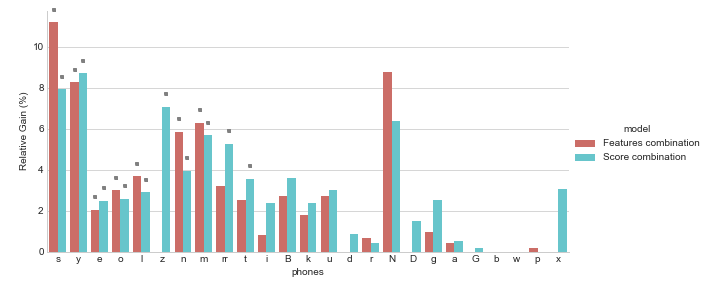
\includegraphics[width=0.8\textwidth]{files/figures/results/relatives/relatives-fusion-systems-dev-all.png}
	\caption{Comparison of performance between Features Combination system and the score combination
	of individual systems in the development set for all phones, sorted descendently by significance
	in the development set. Only the phones marked with (*) were significant in the development set.}
	\label{fig:fusionAllDev}
\end{figure}

\begin{figure}[H]
	\centering
	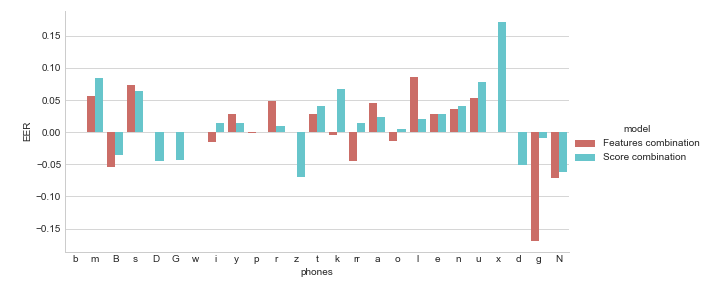
\includegraphics[width=0.8\textwidth]{files/figures/results/relatives/relative-fusion-systems-heldout-all.png}
	\caption{Comparison of performance between Features Combination system and the score combination
	of individual systems in the test set for all phones, sorted descendently by significance
	in the development set. Only the phones marked with (*) were significant in the development set.}
	\label{fig:fusionAllHeldout}
\end{figure}


\printbibliography
 
\end{document}